%% LyX 2.3.4.2 created this file.  For more info, see http://www.lyx.org/.
%% Do not edit unless you really know what you are doing.
\documentclass[english,dvipsnames,aspectratio=169]{beamer}
\usepackage{mathptmx}
\usepackage{eulervm}
\usepackage[T1]{fontenc}
\usepackage[latin9]{inputenc}
\usepackage{babel}
\usepackage{amstext}
\usepackage{amssymb}
\usepackage{graphicx}
\usepackage{ifthen}
\usepackage{xcolor}
\usepackage{xspace}
\usepackage{tikz}
\usetikzlibrary{tikzmark}
\usetikzlibrary{calc}
\usepackage{pgfplots}
%\pgfplotsset{compat=1.17}
\usepackage{booktabs}
\usepackage{xpatch}

\xpatchcmd{\itemize}
  {\def\makelabel}
  {\ifnum\@itemdepth=1\relax
     \setlength\itemsep{2ex}% separation for first level
   \else
     \ifnum\@itemdepth=2\relax
       \setlength\itemsep{1ex}% separation for second level
     \else
       \ifnum\@itemdepth=3\relax
         \setlength\itemsep{0.5ex}% separation for third level
   \fi\fi\fi\def\makelabel
  }
 {}
 {}

\ifx\hypersetup\undefined
  \AtBeginDocument{%
    \hypersetup{unicode=true,pdfusetitle,
 bookmarks=true,bookmarksnumbered=false,bookmarksopen=false,
 breaklinks=false,pdfborder={0 0 0},pdfborderstyle={},backref=false,colorlinks=true,
 allcolors=NYUPurple,urlcolor=LightPurple}
  }
\else
  \hypersetup{unicode=true,pdfusetitle,
 bookmarks=true,bookmarksnumbered=false,bookmarksopen=false,
 breaklinks=false,pdfborder={0 0 0},pdfborderstyle={},backref=false,colorlinks=true,
 allcolors=NYUPurple,urlcolor=LightPurple}
\fi

\makeatletter

%%%%%%%%%%%%%%%%%%%%%%%%%%%%%% LyX specific LaTeX commands.
%% Because html converters don't know tabularnewline
\providecommand{\tabularnewline}{\\}

%%%%%%%%%%%%%%%%%%%%%%%%%%%%%% Textclass specific LaTeX commands.
% this default might be overridden by plain title style
\newcommand\makebeamertitle{\frame{\maketitle}}%
% (ERT) argument for the TOC
\AtBeginDocument{%
  \let\origtableofcontents=\tableofcontents
  \def\tableofcontents{\@ifnextchar[{\origtableofcontents}{\gobbletableofcontents}}
  \def\gobbletableofcontents#1{\origtableofcontents}
}

%%%%%%%%%%%%%%%%%%%%%%%%%%%%%% User specified LaTeX commands.
\usetheme{CambridgeUS} 
\beamertemplatenavigationsymbolsempty


% Set Color ==============================
\definecolor{NYUPurple}{RGB}{87,6,140}
\definecolor{LightPurple}{RGB}{165,11,255}


\setbeamercolor{title}{fg=NYUPurple}
\setbeamercolor{frametitle}{fg=NYUPurple}

\setbeamercolor{background canvas}{fg=NYUPurple, bg=white}
\setbeamercolor{background}{fg=black, bg=NYUPurple}

\setbeamercolor{palette primary}{fg=black, bg=gray!30!white}
\setbeamercolor{palette secondary}{fg=black, bg=gray!20!white}
\setbeamercolor{palette tertiary}{fg=gray!20!white, bg=NYUPurple}

\setbeamertemplate{headline}{}
\setbeamerfont{itemize/enumerate body}{}
\setbeamerfont{itemize/enumerate subbody}{size=\normalsize}
\setbeamerfont{itemize/enumerate subsubbody}{size=\normalsize}

\setbeamercolor{parttitle}{fg=NYUPurple}
\setbeamercolor{sectiontitle}{fg=NYUPurple}
\setbeamercolor{sectionname}{fg=NYUPurple}
\setbeamercolor{section page}{fg=NYUPurple}
%\setbeamercolor{description item}{fg=NYUPurple}
%\setbeamercolor{block title}{fg=NYUPurple}

\setbeamertemplate{blocks}[rounded][shadow=false]
\setbeamercolor{block body}{bg=normal text.bg!90!NYUPurple}
\setbeamercolor{block title}{bg=NYUPurple!30, fg=NYUPurple}



\AtBeginSection[]{
  \begin{frame}
  \vfill
  \centering
\setbeamercolor{section title}{fg=NYUPurple}
 \begin{beamercolorbox}[sep=8pt,center,shadow=true,rounded=true]{title}
    \usebeamerfont{title}\usebeamercolor[fg]{title}\insertsectionhead\par%
  \end{beamercolorbox}
  \vfill
  \end{frame}
}

\makeatother

\setlength{\parskip}{\medskipamount} 

\input ../macros

\begin{document}
\input ../rosenberg-macros

\title[DS-GA 1003]{SVM Dual Problem}
\author{He He}
\date{Feb 23, 2021}
\institute{CDS, NYU}

\makebeamertitle
\mode<article>{Just in article version}

\begin{frame}{SVM as a Quadratic Program}
\begin{itemize}
\item The SVM optimization problem is equivalent to
\begin{eqnarray*}
    \textrm{minimize}_{w, \xi} &  & \frac{1}{2}||w||^{2}+\frac{c}{n}\sum_{i=1}^{n}\xi_{i}\\
\textrm{subject to} &  & -\xi_{i}\le0\;\mbox{for }i=1,\ldots,n\\
 &  & \left(1-y_{i}\left[w^{T}x_{i}+b\right]\right)-\xi_{i}\le0\;\mbox{for }i=1,\ldots,n
\end{eqnarray*}

\item Differentiable objective function
\item $n+d+1$ unknowns and $2n$ affine constraints.
\item A \textbf{quadratic program} that can be solved by any off-the-shelf QP solver. 
\item Let's learn more by examining the dual.
\end{itemize}
\end{frame}

\section{Why Do We Care About the Dual?}

\begin{frame}{The Lagrangian}

The general {[}inequality-constrained{]} optimization problem is:
\begin{eqnarray*}
\textrm{minimize} &  & f_{0}(x)\\
\textrm{subject to} &  & f_{i}(x)\le0,\;\;i=1,\ldots,m
\end{eqnarray*}

\begin{definition}
The \textbf{Lagrangian} for this optimization problem is
\[
L(x,\lambda)=f_{0}(x)+\sum_{i=1}^{m}\lambda_{i}f_{i}(x).
\]
\end{definition}
\begin{itemize}
    \setlength\itemsep{1ex}
    \item $\lambda_{i}$'s are called \textbf{Lagrange multipliers} (also called the \textbf{dual variables}). 
    \item Weighted sum of the objective and constraint functions
    \item Hard constraints $\rightarrow$ soft constraints
\end{itemize}
\end{frame}

\begin{frame}
    {Lagrange Dual Function}
    \begin{definition}
        The \textbf{Lagrange dual function} is
        $$
        g(\lambda) = \inf_x L(x, \lambda)
        = \inf_x \p{f_{0}(x)+\sum_{i=1}^{m}\lambda_{i}f_{i}(x)}
        $$
    \end{definition}
    \begin{itemize}
        \item $g(\lambda)$ is \hl{concave} (infimum of affine functions)
        \item \textbf{Lower bound property}: if $\lambda \succeq 0$, $g(\lambda) \le p^*$ where $p^*$ is the optimal value of the optimization problem.
        \item $g(\lambda)$ can be $-\infty$ (uninformative lower bound)
    \end{itemize}
\end{frame}

\begin{frame}{The Primal and the Dual}
\begin{itemize}
\item For any \textbf{primal form }optimization problem,
\begin{eqnarray*}
\textrm{minimize} &  & f_{0}(x)\\
\textrm{subject to} &  & f_{i}(x)\le0,\;\;i=1,\ldots,m,
\end{eqnarray*}
there is a recipe for constructing a corresponding \textbf{Lagrangian
dual problem:}
\begin{eqnarray*}
\textrm{maximize} &  & g(\lambda)\\
\textrm{subject to} &  & \lambda_{i}\ge0,\;\;i=1,\ldots,m,
\end{eqnarray*}

\item The dual problem is always a convex optimization problem.
\item The dual variables often have interesting and relevant interpretations.
\item The dual variables provide certificate for optimality.
\end{itemize}
\end{frame}

\begin{frame}{Weak Duality}
We always have \textbf{weak duality: }$p^{*}\ge d^{*}$.

\begin{center}
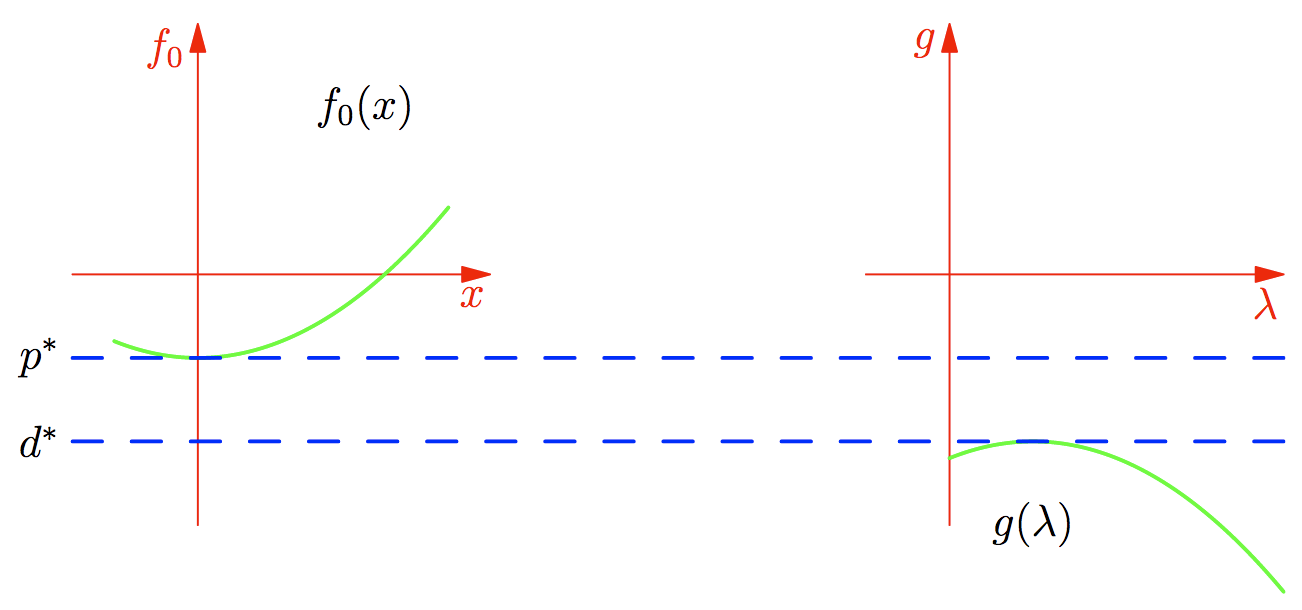
\includegraphics[height=0.6\textheight]{figures/weak-duality}
\par\end{center}

\let\thefootnote\relax\footnotetext{\tiny{Plot courtesy of Brett Bernstein.}}
\end{frame}

\begin{frame}{Strong Duality}

For some problems, we have \textbf{strong duality}: $p^{*}=d^{*}$.

\begin{center}
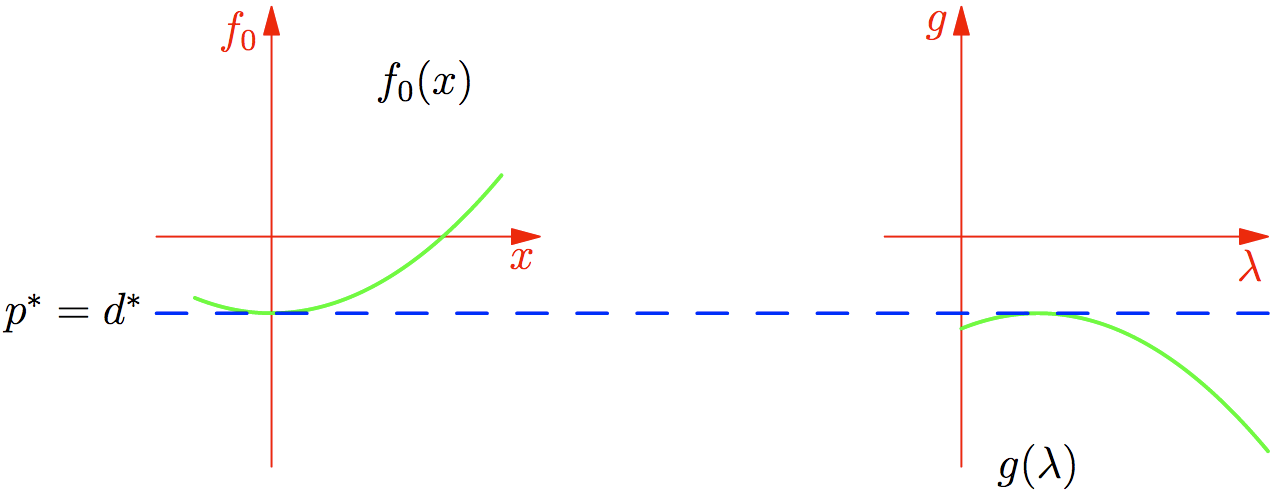
\includegraphics[height=0.6\textheight]{figures/strong-duality}
\par\end{center}

\vspace{-1em}
For convex problems, strong duality is fairly typical. 

\let\thefootnote\relax\footnotetext{\tiny{Plot courtesy of Brett Bernstein.}}
\end{frame}

\begin{frame}{Complementary Slackness}
\begin{itemize}
    \item \hl{Assume strong duality}. Let $x^{*}$ be primal optimal and $\lambda^{*}$ be dual optimal.
Then:
\begin{eqnarray*}
f_{0}(x^{*}) & = & g(\lambda^{*})=\inf_{x}\,L(x,\lambda^{*})\text{\quad(strong duality and definition)}\\
& \le & L(x^{*},\lambda^{*})\\
& = & f_{0}(x^{*})+\sum_{i=1}^{m}{\lambda_{i}^{*}f_{i}(x^{*})}\\
& \le & f_{0}(x^{*}).
\end{eqnarray*}

\end{itemize}
Each term in sum $\sum_{i=1}\lambda_{i}^{*}f_{i}(x^{*})$ must actually
be $0$. That is
\[
    \lambda_i > 0 \implies f_i(x^*) = 0 \quad\text{and}\quad
    f_i(x^*) < 0 \implies \lambda_i = 0 \quad \forall i
\]
This condition is known as \textbf{complementary slackness}. 
\end{frame}

\section{The SVM Dual Problem}
\begin{frame}{SVM Lagrange Multipliers}
    \vspace{-2em}
\begin{eqnarray*}
\textrm{minimize} &  & \frac{1}{2}||w||^{2}+\frac{c}{n}\sum_{i=1}^{n}\xi_{i}\\
\textrm{subject to} &  & -\xi_{i}\le0\quad\mbox{for }i=1,\ldots,n\\
 &  & \left(1-y_{i}\left[w^{T}x_{i}+b\right]\right)-\xi_{i}\le0\quad\mbox{for }i=1,\ldots,n
\end{eqnarray*}

\begin{center}
\begin{tabular}{|c|c|}
\hline 
Lagrange Multiplier & Constraint\tabularnewline
\hline 
\hline 
$\lambda_{i}$ & -$\xi_{i}\le0$\tabularnewline
\hline 
$\alpha_{i}$ & $\left(1-y_{i}\left[w^{T}x_{i}+b\right]\right)-\xi_{i}\le0$\tabularnewline
\hline 
\end{tabular}
\par\end{center}

\[
L(w,b,\xi,\alpha,\lambda)=\frac{1}{2}||w||^{2}+\frac{c}{n}\sum_{i=1}^{n}\xi_{i}+\sum_{i=1}^{n}\alpha_{i}\left(1-y_{i}\left[w^{T}x_{i}+b\right]-\xi_{i}\right)+\sum_{i=1}^{n}\lambda_{i}\left(-\xi_{i}\right)
\]

    \head{Dual optimum value}:
    $d^* = \sup_{\alpha,\lambda\succeq0}\inf_{w,b,\xi}L(w,b,\xi,\alpha,\lambda)$
\end{frame}

\begin{frame}
    {Strong Duality by Slater's Constraint Qualification}
The SVM optimization problem:
\begin{eqnarray*}
\textrm{minimize} &  & \frac{1}{2}||w||^{2}+\frac{c}{n}\sum_{i=1}^{n}\xi_{i}\\
\textrm{subject to} &  & -\xi_{i}\le0\;\mbox{for }i=1,\ldots,n\\
 &  & \left(1-y_{i}\left[w^{T}x_{i}+b\right]\right)-\xi_{i}\le0\;\mbox{for }i=1,\ldots,n
\end{eqnarray*}

Slater's constraint qualification:\\
    \begin{itemize}
\item Convex problem + affine constraints $\implies$strong duality iff
problem is feasible 
\item Do we have a feasible point?
    \note[item]{Constraints are satisfied by $w=b=0$ and $\xi_{i}=1$ for $i=1,\ldots,n$}
\item For SVM, we have strong duality.
    \end{itemize}
\end{frame}

%\begin{frame}
%    {KKT Conditions}
%    For \hl{convex} problems, if \hl{Slater condition} is satisfied, then \textbf{KKT conditions} provide \hl{necessary and sufficient} conditions for the optimal solution.
%    \begin{itemize}
%        \item Primal constraints: $f_i(x) \le 0 \quad \forall i$
%        \item Dual constraints: $\lambda \succeq 0$
%        \item Complementary slackness: $\lambda_i f_i(x)=0$
%        \item First-order condition:
%            $$
%            \frac{\partial}{\partial x} L(x, \lambda) = 0
%            $$
%    \end{itemize}
%\end{frame}

\begin{frame}{SVM Dual Function: First Order Conditions}

Lagrange dual function is the inf over primal variables of $L$: 
\begin{eqnarray*}
 &  & g(\alpha,\lambda)=\inf_{w,b,\xi}L(w,b,\xi,\alpha,\lambda)\\
 & = & \inf_{w,b,\xi}\left[\frac{1}{2}w^{T}w+\sum_{i=1}^{n}\xi_{i}\left(\frac{c}{n}-\alpha_{i}-\lambda_{i}\right)+\sum_{i=1}^{n}\alpha_{i}\left(1-y_{i}\left[w^{T}x_{i}+b\right]\right)\right]
\end{eqnarray*}
    \note[item]{How do we solve the minimization problem?}
    \note[item]{Is it convex? [yes, quadratic term]}

\pause{}
    \vspace{-2em}
\begin{eqnarray*}
\partial_{w}L=0 & \iff & w-\sum_{i=1}^{n}\alpha_{i}y_{i}x_{i}=0\;\iff\;\boxed{w=\sum_{i=1}^{n}\alpha_{i}y_{i}x_{i}}\\
\partial_{b}L=0 & \iff & -\sum_{i=1}^{n}\alpha_{i}y_{i}=0\;\iff\;\boxed{\sum_{i=1}^{n}\alpha_{i}y_{i}=0}\\
\partial_{\xi_{i}}L=0 & \iff & \frac{c}{n}-\alpha_{i}-\lambda_{i}=0\;\iff\;\boxed{\alpha_{i}+\lambda_{i}=\frac{c}{n}}
\end{eqnarray*}
\end{frame}

\begin{frame}{SVM Dual Function}
\begin{itemize}
    \setlength\itemsep{1ex}
\item Substituting these conditions back into $L$, the second term disappears.
\item First and third terms become 
\begin{eqnarray*}
\frac{1}{2}w^{T}w & = & \frac{1}{2}\sum_{i,j=1}^{n}\alpha_{i}\alpha_{j}y_{i}y_{j}x_{i}^{T}x_{j}\\
\sum_{i=1}^{n}\alpha_{i}(1-y_{i}\left[w^{T}x_{i}+b\right]) & = & \sum_{i=1}^{n}\alpha_{i}-\sum_{i,j=1}^{n}\alpha_{i}\alpha_{j}y_{i}y_{j}x_{j}^{T}x_{i}-b\underbrace{\sum_{i=1}^{n}\alpha_{i}y_{i}}_{=0}.
\end{eqnarray*}

        \vspace{-2ex}
\item Putting it together, the dual function is 
\[
g(\alpha,\lambda)=\begin{cases}
\sum_{i=1}^{n}\alpha_{i}-\frac{1}{2}\sum_{i,j=1}^{n}\alpha_{i}\alpha_{j}y_{i}y_{j}x_{j}^{T}x_{i} & \substack{\substack{\sum_{i=1}^{n}\alpha_{i}y_{i}=0\\
\alpha_{i}+\lambda_{i}=\frac{c}{n}\mbox{, all }i
}
}
\\
-\infty & \mbox{otherwise.}
\end{cases}
\]
\end{itemize}
\end{frame}

\begin{frame}{SVM Dual Problem}
\begin{itemize}
\item The \textbf{dual function} is
\[
g(\alpha,\lambda)=\begin{cases}
\sum_{i=1}^{n}\alpha_{i}-\frac{1}{2}\sum_{i,j=1}^{n}\alpha_{i}\alpha_{j}y_{i}y_{j}x_{j}^{T}x_{i} & \substack{\substack{\sum_{i=1}^{n}\alpha_{i}y_{i}=0\\
\alpha_{i}+\lambda_{i}=\frac{c}{n}\mbox{, all }i
}
}
\\
-\infty & \mbox{otherwise.}
\end{cases}
\]


\item The \textbf{dual problem }is $\sup_{\alpha,\lambda\succeq0}g(\alpha,\lambda)$:
\begin{eqnarray*}
\sup_{\alpha,\lambda} &  & \sum_{i=1}^{n}\alpha_{i}-\frac{1}{2}\sum_{i,j=1}^{n}\alpha_{i}\alpha_{j}y_{i}y_{j}x_{j}^{T}x_{i}\\
\mbox{s.t.} &  & \sum_{i=1}^{n}\alpha_{i}y_{i}=0\\
 & \quad & \alpha_{i}+\lambda_{i}=\frac{c}{n}\quad\alpha_{i},\lambda_{i}\ge0,\;i=1,\ldots,n
\end{eqnarray*}
 
\end{itemize}
\end{frame}

\section{Insights from the Dual Problem}
\begin{frame}{The SVM Dual Solution}
\begin{itemize}
\item We found the SVM dual problem can be written as:
\begin{eqnarray*}
\sup_{\alpha} &  & \sum_{i=1}^{n}\alpha_{i}-\frac{1}{2}\sum_{i,j=1}^{n}\alpha_{i}\alpha_{j}y_{i}y_{j}x_{j}^{T}x_{i}\\
\mbox{s.t.} &  & \sum_{i=1}^{n}\alpha_{i}y_{i}=0\\
 & \quad & \alpha_{i}\in\left[0,\frac{c}{n}\right]\;i=1,\ldots,n.
\end{eqnarray*}
\end{itemize}

\begin{itemize}
\item Given solution $\alpha^{*}$ to dual, primal solution is $w^{*}=\sum_{i=1}^{n}\alpha_{i}^{*}y_{i}x_{i}$. 
\item The solution is in the space spanned by the inputs.
\item Note $\alpha_{i}^{*}\in[0,\frac{c}{n}]$. So $c$ controls max weight
on each example. (\textbf{Robustness}!)
        \begin{itemize}
            \item What's the relation between $c$ and regularization?
        \end{itemize}
\end{itemize}
\end{frame}

\begin{frame}{Complementary Slackness Conditions}
\begin{itemize}
\item Recall our primal constraints and Lagrange multipliers:
\end{itemize}
\begin{center}
\begin{tabular}{|c|c|}
\hline 
Lagrange Multiplier & Constraint\tabularnewline
\hline 
\hline 
$\lambda_{i}$ & -$\xi_{i}\le0$\tabularnewline
\hline 
$\alpha_{i}$ & $\left(1-y_{i}f(x_{i})\right)-\xi_{i}\le0$\tabularnewline
\hline 
\end{tabular}
\par\end{center}

\begin{itemize}
\item Recall first order condition $\del_{\xi_{i}}L=0$ gave us $\lambda_{i}^{*}=\frac{c}{n}-\alpha_{i}^{*}$.
\item By strong duality, we must have \textbf{complementary slackness}:
\begin{align*}
\alpha_{i}^{*}\left(1-y_{i}f^{*}(x_{i})-\xi_{i}^{*}\right) & =0\\
\lambda_{i}^{*}\xi_{i}^{*}=\left(\frac{c}{n}-\alpha_{i}^{*}\right)\xi_{i}^{*} & =0
\end{align*}
\end{itemize}
\end{frame}

\begin{frame}{Consequences of Complementary Slackness}
By strong duality, we must have \textbf{complementary slackness}.
\begin{align*}
\alpha_{i}^{*}\left(1-y_{i}f^{*}(x_{i})-\xi_{i}^{*}\right) & =0\\
\left(\frac{c}{n}-\alpha_{i}^{*}\right)\xi_{i}^{*} & =0
\end{align*}

Recall ``\textbf{slack variable}'' $\xi_{i}^{*}=\max\left(0,1-y_{i}f^{*}(x_{i})\right)$
is the hinge loss on $\left(x_{i},y_{i}\right)$.
\begin{itemize}
\item If $y_{i}f^{*}(x_{i})>1$ then the margin loss is $\xi_{i}^{*}=0$,
and we get $\alpha_{i}^{*}=0$.
\item If $y_{i}f^{*}(x_{i})<1$ then the margin loss is $\xi_{i}^{*}>0$,
so $\alpha_{i}^{*}=\frac{c}{n}$. 

\item If $\alpha_{i}^{*}=0$, then $\xi_{i}^{*}=0$, which implies no loss,
so $y_{i}f^{*}(x)\ge1$.

\item If $\alpha_{i}^{*}\in\left(0,\frac{c}{n}\right)$, then $\xi_{i}^{*}=0$,
which implies $1-y_{i}f^{*}(x_{i})=0$.
\end{itemize}
\end{frame}

\begin{frame}{Complementary Slackness Results: Summary}
If $\alpha^{*}$ is a solution to the dual problem, then primal solution
is 
\[
w^{*}=\sum_{i=1}^{n}\alpha_{i}^{*}y_{i}x_{i}
    \quad \text{where} \alpha_{i}^{*}\in[0,\frac{c}{n}] .
\]

    Relation between margin and example weights ($\alpha_i$'s):
\begin{eqnarray*}
\alpha_{i}^{*}=0 & \implies & y_{i}f^{*}(x_{i})\ge1\\
\alpha_{i}^{*}\in\left(0,\frac{c}{n}\right) & \implies & y_{i}f^{*}(x_{i})=1\\
\alpha_{i}^{*}=\frac{c}{n} & \implies & y_{i}f^{*}(x_{i})\le1
\end{eqnarray*}
\begin{eqnarray*}
y_{i}f^{*}(x_{i})<1 & \implies & \alpha_{i}^{*}=\frac{c}{n}\\
y_{i}f^{*}(x_{i})=1 & \implies & \alpha_{i}^{*}\in\left[0,\frac{c}{n}\right]\\
y_{i}f^{*}(x_{i})>1 & \implies & \alpha_{i}^{*}=0
\end{eqnarray*}
\end{frame}

\begin{frame}{Support Vectors}
\begin{itemize}
\item If $\alpha^{*}$ is a solution to the dual problem, then primal solution
is 
\[
w^{*}=\sum_{i=1}^{n}\alpha_{i}^{*}y_{i}x_{i}
\]
with $\alpha_{i}^{*}\in[0,\frac{c}{n}]$. 

\item The $x_{i}$'s corresponding to $\alpha_{i}^{*}>0$ are called \textbf{support
vectors.}

\item Few margin errors or ``on the margin'' examples $\implies$ \hl{sparsity
in input examples}.
\end{itemize}
\end{frame}

\begin{frame}{The Bias Term: $b$}
\begin{itemize}
\item For our SVM primal, the complementary slackness conditions are:
\begin{align}
\alpha_{i}^{*}\left(1-y_{i}\left[x_{i}^{T}w^{*}+b\right]-\xi_{i}^{*}\right) & =0\label{eq:lossNonNegativeSlackCondition-1}\\
\lambda_{i}^{*}\xi_{i}^{*}=\left(\frac{c}{n}-\alpha_{i}^{*}\right)\xi_{i}^{*} & =0\label{eq:marginLossSlackCondition-1}
\end{align}


\item Suppose there's an $i$ such that $\alpha_{i}^{*}\in\left(0,\frac{c}{n}\right)$.

\item \eqref{eq:marginLossSlackCondition-1} implies $\xi_{i}^{*}=0$.

\item \eqref{eq:lossNonNegativeSlackCondition-1} implies 
\begin{eqnarray*}
 &  & y_{i}\left[x_{i}^{T}w^{*}+b^{*}\right]=1\\
 & \iff & x_{i}^{T}w^{*}+b^{*}=y_{i}\mbox{ (use }y_{i}\in\left\{ -1,1\right\} )\\
 & \iff & \boxed{b^{*}=y_{i}-x_{i}^{T}w^{*}}
\end{eqnarray*}
\end{itemize}
\end{frame}

\begin{frame}{The Bias Term: $b$}
\begin{itemize}
\item We get the same $b^{*}$ for any choice of $i$ with $\alpha_{i}^{*}\in\left(0,\frac{c}{n}\right)$ 
\[
b^{*}=y_{i}-x_{i}^{T}w^{*}
\]

\item With numerical error, more robust to average over all eligible $i$'s:
\[
b^{*}=\text{mean}\left\{ y_{i}-x_{i}^{T}w^{*}\mid\alpha_{i}^{*}\in\left(0,\frac{c}{n}\right)\right\} .
\]

\item If there are no $\alpha_{i}^{*}\in\left(0,\frac{c}{n}\right)$?
\begin{itemize}
\item Then we have a \textbf{degenerate SVM training problem}\footnote{See Rifkin et al.'s ``A Note on Support Vector Machine Degeneracy'',
an MIT AI Lab Technical Report.} ($w^{*}=0$).
\end{itemize}
\end{itemize}
\end{frame}


\end{document}
